\newpage

\section{Промышленная экология и безопасность}
\subsection{Анализ опасных и вредных факторов, возникающих при работе на ПЭВМ}
Для обеспечения комфортных условий труда сотрудника организации, рабочее место которого включает ПЭВМ, необходимо выполнение следующие требования\cite{SanPinGigiena}:
\begin{enumerate}
\item требования к ПЭВМ, установленные в СанПин 2.2.2/2.4.1340-03 <<Гигиенические требования к персональным электронно-вычислительным машинам и организации работы>>;
\item требования к помещениям для работы с ПЭВМ;
\item требования к организации и оборудованию рабочих мест с ПЭВМ;
\item требования к микроклимату помещения, установленные в  СанПиН \\2.2.4.548-96 <<Гигиенические требования к микроклимату производственных помещений>>;
\item требования к освещению на рабочих местах, оборудованных ПЭВМ
\item требования к уровням шума и вибрации на рабочих местах, оборудованных ПЭВМ;
\item требования к режиму труда и отдыха.
\end{enumerate}

\subsubsection{Помещение для работы с ПЭВМ}

Ниже приведены основные требования, предъявляемые к помещениям, предназначенным для работы сотрудников с ПЭВМ.

Помещения для эксплуатации ПЭВМ должны иметь естественное и искусственное освещение. Эксплуатация ПЭВМ в помещениях без естественного освещения допускается только при соответствующем обосновании и наличии положительного санитарно-эпидемиологического заключения, выданного в установленном порядке.

Окна в помещениях, где эксплуатируется вычислительная техника, преимущественно должны быть ориентированы на север и северо-восток. Оконные проемы должны быть оборудованы регулируемыми устройствами типа: жалюзи, занавесей, внешних козырьков и др.

Для внутренней отделки интерьера помещений, где расположены ПЭВМ, должны использоваться диффузно-отражающие материалы с коэффициентом отражения для потолка – 0,7 - 0,8; для стен – 0,5 - 0,6; для пола – 0,3 - 0,5.

Полимерные материалы используются для внутренней отделки интерьера помещений с ПЭВМ при наличии санитарно-эпидемиологического заключения.

Помещения, где размещаются рабочие места с ПЭВМ, должны быть оборудованы защитным заземлением (занулением) в соответствии с техническими требованиями по эксплуатации.

\subsubsection{Рабочее место оператора и положение за рабочим местом}
\paragraph{Общие требования}

При размещении рабочих мест с ПЭВМ расстояние между рабочими столами с видеомониторами (в направлении тыла поверхности одного видеомонитора и экрана другого видеомонитора), должно быть не менее 2,0 м, а расстояние между боковыми поверхностями видеомониторов не менее 1,2 м.

Рабочие места с ПЭВМ в помещениях с источниками вредных производственных факторов должны размещаться в изолированных кабинах с организованным воздухообменом. 

Рабочие места с ПЭВМ при выполнении творческой работы, требующей значительного умственного напряжения или высокой концентрации внимания, рекомендуется изолировать друг от друга перегородками 1,5 – 2,0 м.

Экран видеомонитора должен находиться от глаз пользователя на расстоянии 600-700 мм, но не ближе 500 мм с учетом размеров алфавитно-цифровых знаков и символов.

Конструкция рабочего стола должна обеспечивать оптимальное размещение на рабочей поверхности используемого оборудования с учетом его количества и конструктивных особенностей, характера выполняемой работы.

При этом допускается использование рабочих столов различных конструкций, отвечающих современным требованиям эргономики. Поверхность рабочего стола должна иметь коэффициент отражения 0,5 – 0,7.

Конструкция рабочего стула (кресла) должна обеспечивать поддержание рациональной рабочей позы при работе на ПЭВМ, позволять изменять позу с целью снижения статического напряжения мышц шейно-плечевой области и спины для предупреждения развития утомления. Тип рабочего стула (кресла) следует выбирать с учетом роста пользователя, характера и продолжительности работы с ПЭВМ.

Рабочий стул (кресло) должен быть подъемно-поворотным, регулируемым по высоте и углам наклона сиденья и спинки, а также расстоянию спинки от переднего края сиденья, при этом регулировка каждого параметра должна быть независимой, легко осуществляемой и иметь надежную фиксацию.

Поверхность сиденья, спинки и других элементов стула (кресла) должна быть полумягкой, с нескользящим, слабо электризующимся и воздухопроницаемым покрытием, обеспечивающим легкую очистку от загрязнений.

\paragraph{Требования к значениям параметров рабочего места}

Значения параметров рабочего стола приведены в таблице~\ref{bzd:workplace}.

\begin{table}[!htb]
	\caption{Значения параметров рабочего стола}\label{bzd:workplace}
    \centering
    \begin{tabular}{|p{10cm}|p{6cm}|}
        \hline 
        \textbf{Параметры рабочего стола} & \textbf{Значения, мм} \\ 
        \hline 
        Высота рабочей поверхности & регулировка 680-800,
или фиксировано 725 \\ 
        \hline 
        Ширина рабочей поверхности & 1200 \\ 
        \hline 
        Глубина рабочей поверхности & 800 \\ 
        \hline 
        Высота пространства для ног & 750 \\ 
        \hline 
        Ширина пространства для ног & 900 \\ 
        \hline 
        Глубина пространства для ног на уровне колен & 900 \\ 
        \hline 
        Глубина пространства для ног на уровне вытянутых ног & 900 \\ 
        \hline 
        \end{tabular}     
    		
\end{table}

Конструкция рабочего стула (кресла) должна обеспечивать поддержание рациональной рабочей позы при работе на ПЭВМ, позволять изменять позу с целью снижения статического напряжения мышц шейно-плечевой области и спины для предупреждения развития утомления. Тип рабочего стула (кресла) следует выбирать с учетом роста пользователя, характера и продолжительности работы с ПЭВМ.

Рабочий стул (кресло) должен быть подъемно-поворотным, регулируемым по высоте и углам наклона сиденья и спинки, а также расстоянию спинки от переднего края сиденья, при этом регулировка каждого параметра должна быть независимой, легко осуществляемой и иметь надежную фиксацию.

Конструкция рабочего стула должна обеспечивать поверхность сиденья с закругленным передним краем, а также соответствие значений параметров приведённым в таблице~\ref{bzd:workchair}.

\begin{table}[!htb]
	\caption{Значения параметров рабочего стула (кресла)}\label{bzd:workchair}
    \centering
    \begin{tabular}{|p{10cm}|p{6cm}|}
        \hline 
        \textbf{Параметры рабочего стыла (кресла)} & \textbf{Значения} \\ 
        \hline 
        Ширина и глубина поверхности сиденья & не менее 400 мм \\ 
        \hline 
        Высота поверхности сиденья & 400 – 550 мм \\ 
        \hline 
        Угол наклона поверхности сиденья вперед (назад) & до 15 (5) градусов \\ 
        \hline 
        Высота опорной поверхности спинки & 280 – 320 мм \\ 
        \hline 
        Ширина опорной поверхности спинки & не менее 380 мм \\ 
        \hline 
        Радиус кривизны горизонтальной плоскости спинки & 400 мм \\ 
        \hline 
        Угол наклона спинки в вертикальной плоскости & $\pm$ 30 градусов \\ 
        \hline 
        Расстояние спинки от переднего края сиденья & 260 – 400 мм \\ 
        \hline 
        Длина подлокотников & не менее 250 мм \\ 
        \hline 
        Ширина подлокотников & 50 – 70 мм \\ 
        \hline 
        Высота подлокотников над сиденьем & 200 – 260 мм \\ 
        \hline 
        Внутреннее расстояние между подлокотниками & 350 – 500 мм \\ 
        \hline 
        \end{tabular}     
    		
\end{table}

Рабочее место пользователя ПЭВМ следует оборудовать подставкой для ног, имеющей ширину не менее 300 мм, глубину не менее 400 мм, регулировку по высоте в пределах до 150 мм и по углу наклона опорной поверхности подставки до 20 градусов. Поверхность подставки должна быть рифленой и иметь по переднему краю бортик высотой 10 мм.

Клавиатуру следует располагать на поверхности стола на расстоянии 100 – 300 мм от края, обращенного к пользователю или на специальной, регулируемой по высоте рабочей поверхности, отделенной от основной столешницы.

\paragraph{Микроклимат}
Оптимальные микроклиматические условия установлены по критериям оптимального теплового и функционального состояния человека. Они обеспечивают общее и локальное ощущение теплового комфорта в течение 8-часовой рабочей смены при минимальном напряжении механизмов терморегуляции, не вызывают отклонений в состоянии здоровья, создают предпосылки для высокого уровня работоспособности и являются предпочтительными на рабочих местах.
 
В помещениях, в которых работа с использованием ПЭВМ является основной и связана с нервно-эмоциональным напряжением, должны обеспечиваться оптимальные параметры микроклимата. 

В санитарных нормах СанПиН 2.2.2/2.4.1340-03 установлены величины параметров микроклимата, создающие комфортные условия\cite{SanPinAeroIon}. Эти нормы устанавливаются в зависимости от времени года, характера трудового процесса и характера производственного помещения (значительные или незначительные тепловыделения). В данном дипломном проекте рассматриваются условия труда пользователей ПЭВМ, которые относятся к категории Iа, (интенсивность энергозатрат до 120 ккал/ч (до 139 Вт), работа, производимая сидя и сопровождающиеся незначительным физическим напряжением). Величины микроклиматических параметров приведены в таблице~\ref{bzd:microclimat}.

\begin{table}[!htb]
	\caption{Оптимальные параметры микроклимата в помещении}\label{bzd:microclimat}
    \centering
	\begin{tabular}{|p{2cm}|p{2,5cm}|p{2,5cm}|p{3cm}|p{3cm}|p{2,7cm}|}
	\hline 
	Период года & 
	Категория работ по уровню & 
	Темпера тура воздуха,$^{\circ}С$ &
	Температура поверхно стей,$^{\circ}С$ &
	Относи\par тельная влажность воздуха, \% & 
	Скорость движения воздуха, м/с \\ 
	\hline 
	Холод-\par ный & Ia (до 139) & 22-24 & 21-25 & 60-40 & 0,1 \\ 
	\hline 
	Теплый & Ia (до 139) & 23-25 & 22-26 & 60-40 & 0,1\\ 
	\hline 
	\end{tabular} 
    		
\end{table}

Перепады температуры воздуха по высоте и по горизонтали, а также изменения температуры воздуха в течение смены при обеспечении оптимальных величин микроклимата на рабочих местах не должны превышать 2 $^{\circ}С$.

\paragraph{Аэроионный состав воздуха}

В связи с тем, что разработка данного дипломного проекта производилась в помещении, в отделке и (или) меблировке которых используются синтетические материалы или покрытия, способные накапливать электростатический заряд; а так же - в которых эксплуатируется оборудование, способное создавать электростатические поля, включая видеодисплейные терминалы и прочие виды оргтехники, то необходимо учесть действующие <<Гигиенические требования к аэроионному составу воздуха производственных и общественных помещений>> (СанПиН 2.2.4.1294-03), а именно:

\begin{enumerate}
\item Нормируемые показатели аэроионного состава воздуха
	\begin{enumerate}
	\item Аэроионный состав воздуха устанавливается в зависимости от процессов ионизации и деионизации.
	\item Нормируемыми показателями аэроионного состава воздуха производственных и общественных помещений являются:
		\begin{itemize}
			\item концентрации аэроионов (минимально допустимая и максимально допустимая) обеих полярностей р+. р-, определяемые как количество аэроионов в одном кубическом сантиметре воздуха (ион/см\textsuperscript{3});
			\item коэффициент униполярности Y (минимально допустимый и максимально допустимый) определяемый как отношение концентрации аэроионов положительной полярности к концентрации аэроионов отрицательной полярности.
		\end{itemize}
		\item Минимально и максимально допустимые значения нормируемых показателей определяют диапазоны концентраций аэроионов обеих полярностей и коэффициента униполярности, отклонения от которых могут привести к неблагоприятным последствиям для здоровья человека.
		\item Значения нормируемых показателей концентраций аэроионов и коэффициента униполярности приведены в таблице~\ref{bzd:aeroion}.

\begin{table}[!htb]
			\caption{Нормируемые показатели аэроионов и коэффициенты униполярности}\label{bzd:aeroion}
		    \centering
			\begin{tabular}{|p{4cm}|p{3,5cm}|p{3,5cm}|p{3,5cm}|}
			\hline 
			Нормируемые показатели & 
			Концентрация n+ (ион/см\textsuperscript{3}) & 
			Концентрация n-(ион/см\textsuperscript{3}) & 
			Коэффициент униполярности Y\\ 
			\hline 
			Минимально допустимые & n+ $\geq$ 400 &  n- $\geq$ 400 &  0,4 $\leq$ Y $\leq$ 1,0\\ 
			\hline 
			Максимально допустимые & n+ $<$ 50000 & n- $<$ 50000 & ~\ \\ 
			\hline 
			\end{tabular} 
		    		
		\end{table}
		
		\item В зонах дыхания персонала на рабочих местах, где имеются источники электростатических полей (видеодисплейные терминалы или другие виды оргтехники) допускается отсутствие аэроионов положительной полярности.
		\item Степени вредности отклонений от означенных диапазонов концентрации аэроионов и коэффициента униполярности определяются в соответствии с классификацией условий труда по аэроионному составу воздуха.
		\item В лечебных целях могут применяться другие показатели аэроионного состава воздуха если это предусмотрено утвержденными в установленном порядке методиками лечения или применения аэроионизаторов.
	\end{enumerate}
\item Требования к проведению контроля аэроионного состава воздуха
	\begin{enumerate}
	\item Контроль аэроионного состава воздуха осуществляется в следующих случаях: 
		\begin{itemize}
		\item в порядке планового контроля не реже одного раза в год;
		\item при аттестации рабочих мест;
		\item при вводе в эксплуатацию оборудования либо материалов, способных создавать или накапливать электростатический заряд \\(включая видеодисплейные терминалы и прочие виды оргтехники);
		\item при оснащении рабочих мест аэроионизаторами или деионизаторами.
		\end{itemize}
	\item Проведение контроля аэроионного состава воздуха помещений следует осуществлять непосредственно на рабочих местах в зонах дыхания персонала и в соответствии с утвержденными в установленном порядке методиками контроля.
	\end{enumerate}
\item Требования к способам и средствам нормализации аэроионного состава воздуха
	\begin{enumerate}
	\item Если в результате контроля аэроионного состава воздуха выявляется его несоответствие нормированным показателям, рекомендуется осуществление его нормализации.
	\item Осуществление нормализации аэроионного состава воздуха рекомендуется производить на протяжении всего времени пребывания человека на рабочем месте.
	\item Для нормализации аэроионного состава воздуха следует применять соответствующие, прошедшие санитарно-эпидемиологическую оценку и имеющие действующее санитарно-эпидемиологическое заключение аэроионизаторы или деионизаторы предназначенные для использования в санитарно-гигиенических целях.
	\item Санитарно-эпидемиологическая оценка и эксплуатация аэроионизаторов и деионизаторов осуществляется в установленном порядке.

	\end{enumerate}
\end{enumerate}

\paragraph{Шум и вибрация}

На рабочем месте пользователя ПЭВМ источниками шума, как правило, разговаривающие люди, внешний шум, компьютер, принтер, вентиляционное оборудование. Основными источниками внешнего шума являются транспортные потоки на улицах и дорогах.

Нормируемыми параметрами постоянного шума являются уровни звукового давления L, дБ, в октавных полосах частот со среднегеометрическими частотами 31,5; 63; 125; 250; 500; 1000; 2000; 4000 и 8000 Гц. Для ориентировочных расчетов допускается использование уровней звука LА, дБА.

Допустимые уровни звукового давления, уровня звука и эквивалентные уровни звука на рабочих местах должны соответствовать требованиям СанПиН 2.2.2/2.4.1340-03.

Показатели нормируемых уровней шума для помещений офисов, рабочих помещений и кабинетов административных зданий (помещения, где могут располагаться рабочие места сотрудников – разработчиков и эксплуататоров проектируемой системы) приведены в таблице .

Основным из механических факторов производственной среды является вибрация. Она не только вредно действуют на организм, но и мешают человеку выполнять как мыслительные, так и двигатель¬ные операции. 

\begin{table}[!htb]
	\caption{Параметры производственного шума}\label{bzd:noize}
    \centering
	\begin{tabular}{|p{1cm}|p{1cm}|p{1cm}|p{1cm}|p{1cm}|p{1cm}|p{1cm}|p{1cm}|p{1cm}|p{2cm}|}
	\hline 
	\multicolumn{9}{|p{12cm}|}{Уровни звукового давления в октавных полосах со среднегеометрическими частотами} & Уровни звука в дБА \\ 
	\hline 
	31,5 Гц & 63 Гц & 125 Гц & 250 Гц & 500 Гц & 1000 Гц & 2000 Гц & 4000 Гц & 8000 Гц & ~\ \\ 
	\hline 
	86 дБ & 71 дБ & 61 дБ & 54 дБ & 49 дБ & 45 дБ & 42 дБ & 40 дБ & 38 дБ & 50 \\ 
	\hline 
	\end{tabular} 
    		
\end{table}

Шум считают в пределах нормы, когда он как по эквивалентному, так и по максимальному уровню не превышает установленные нормативные значения.
Допустимые уровни шума от внешних источников в помещениях установлены при условии обеспечения нормативного воздухообмена, т.е при отсутствии принудительной системы вентиляции или кондиционирования воздуха, должны выполняться при условии открытых форточек или иных устройств, обеспечивающих приток воздуха.

Защита от шума строительно-акустическими методами должна обеспечиваться:
\begin{itemize}
\item рациональным архитектурно-планировочным решением здания;
\item применением ограждающих конструкций, обеспечивающих нормативную звукоизоляцию;
\item применением звукопоглощающих облицовок в помещении здания;
\item применением глушителей шума в системах принудительной вентиляции и кондиционирования воздуха;
\item виброизоляцией инженерного и санитарно-технического оборудования зданий.
\end{itemize}

\subsubsection{Освещение}
\paragraph{Общие требования}

Ниже приведены основные требования, предъявляемые к освещению помещений, предназначенных для работы сотрудников с ПЭВМ.

Рабочие столы следует размещать таким образом, чтобы видеодисплейные терминалы были ориентированы боковой стороной к световым проемам, чтобы естественный свет падал преимущественно слева.

Искусственное освещение в помещениях для эксплуатации ПЭВМ должно осуществляться системой общего равномерного освещения. В производственных помещениях, в случаях основной работы с документами, можно применять системы комбинированного освещения (к общему освещению дополнительно устанавливаются светильники местного освещения, предназначенные для освещения зоны расположения документов).

Освещенность на поверхности стола в зоне размещения рабочего документа должна быть 300 – 500 лк. Освещение не должно создавать бликов на поверхности экрана. Освещенность поверхности экрана не должна быть более 300 лк.

Следует ограничивать прямую блесткость от источников освещения, при этом яркость светящихся поверхностей (окна, светильники и др.), находящихся в поле зрения, должна быть не более 200 кд/м\textsuperscript{2}.

Следует ограничивать отраженную блесткость на рабочих поверхностях (экран, стол, клавиатура и др.) за чет правильного выбора типов светильников и расположения рабочих мест по отношению к источникам естественного и искусственного освещения, при этом яркость бликов на экране ПЭВМ не должна превышать 40 кд/м\textsuperscript{2} и яркость потолка не должна превышать 200 кд/м\textsuperscript{2}.

Яркость светильников общего освещения в зоне углов излучения от 50 до 90 градусов с вертикалью в продольной и поперечной плоскостях должна составлять не более 200 кд/м\textsuperscript{2}, защитный угол светильников должен быть не менее 40 градусов.

 Светильники местного освещения должны иметь не просвечивающий отражатель с защитным углом не менее 40 градусов.
 
 Следует ограничивать неравномерность распределения яркости в поле зрения пользователя ПЭВМ, при этом соотношение яркости между рабочими поверхностями не должно превышать 3:1 – 5:1, а между рабочими поверхностями и поверхностями стен и оборудования 10:1.

В качестве источников света при искусственном освещении следует применять преимущественно люминесцентные лампы типа ЛБ. При устройстве отраженного освещения в производственных и административно-\\общественных помещениях допускается применение металлогалогенных ламп. В светильниках местного освещения допускается применение ламп накаливания, в том числе галогенные.

Для освещения помещений с ПЭВМ следует применять светильники с зеркальными параболическими решетками, укомплектованными электронными пуско-\\регулирующими аппаратами. Допускается использование многоламповых светильников с электромагнитными пуско-регулирующими аппаратами, состоящими из равного числа опережающих и отстающих ветвей.

Применение светильников без рассеивателей и экранирующих решеток не допускается. При выполнениии работы использовались лампы с экранирующими решетками.

Общее освещение при использовании люминесцентных светильников следует выполнять в виде сплошных или прерывистых линий светильников, расположенных сбоку от рабочих мест, параллельно линии зрения пользователя при рядном расположении видеодисплейных терминалов. 

Коэффициент запаса (Кз) для осветительных установок общего освещения должен приниматься равным 1,4.

Коэффициент пульсации не должен превышать 5\%.

Для обеспечения нормируемых значений освещенности в помещениях для использования ПЭВМ проводится чистка стекол оконных рам и светильников не реже двух раз в год и своевременную замену перегоревших ламп.

\subsubsection{Расчёт освещения}
\paragraph{Искусственное освещение}

Так как минимальным объектом различения при работе с ПЭВМ является пиксель, размер которого составляет 0.28мм, то выполняемый вид работ считаем зрительной работой очень высокой точности\cite{SP52}. 

Нормы для искусственного освещения приведены в таблице~\ref{bzd:svet}.

\begin{table}[!htb]
	\caption{Нормы для искусственного освещения}\label{bzd:svet}
    \centering
	\begin{tabular}{|p{3cm}|p{2,5cm}|p{2cm}|p{2cm}|p{3cm}|p{2cm}|}
	\hline 
	\multirow{2}{3cm}{~\ Характеристика зрительной работы} &
	\multirow{2}{2,5cm}{Размер объекта различения, мм} & 
	\multirow{2}{2cm}{Контраст объекта с фоном} &
	\multirow{2}{2cm}{Фон} &
	\multicolumn{2}{p{5cm}|}{Освещенность, лк}\\ 
	\cline{5-6} 
	 &  &  &  & ~\ Комбинированное освещение &  Общее освещение \\ 
	\hline 
	\multirow{4}{3cm}{Очень высокой точности} &
	\multirow{4}{2,5cm}{0,15 - 0,30} & 
	малый & темный & 4000 & - \\
	\cline{3-6} 
	& & малый & средний & 3000 & 750 \\
	& & средний & темный & 2500 & 600 \\
	\cline{3-6} 
	& & малый & светлый & 2000 & 500 \\
	& & средний & средний & 1500 & 400 \\
	& & большой & темный &  &  \\
	\cline{3-6} 
	& & средний & светлый & 1000 & 300 \\
	& & большой & светлый & 750 & 200 \\
	& & большой & средний &  &  \\
	\hline
	\end{tabular} 
    		
\end{table}

При работе оператора разрабатываемой подсистемы предполагается работа при среднем контрасте и светлом фоне. Таким образом, нормированная минимально-допустимая освещенность при общем освещении составляет 300 лк. 

Основным методом расчета общего равномерного освещения при горизонтальной рабочей поверхности является метод светового потока (коэффициента использования). Необходимый световой поток Фл (лм) от одной лампы накаливания или группы ламп светильника при люминесцентных лампах рассчитывают по формуле \ref{bzd:svetpotok}.

\begin{equation}\label{bzd:svetpotok}
Ф_{осв}=\frac{E_н \cdot S \cdot z \cdot k}{N_c \cdot \eta},
\end{equation}

где $E_н$ – нормированная минимально-допустимая освещенность (лк), которая определяется нормативом (см. таблицу~\ref{bzd:svet}); $S$ — площадь освещаемого помещения (м\textsuperscript{2}); $z$ — коэффициент неравномерности освещения, который зависит от типа ламп (для ламп накаливания и дуговых ртутных ламп — 1,15, для люминесцент¬ных ламп — 1,1); k — коэффициент запаса, соласно \cite{metodaBZD} равен 1,4; $N_c$ — число светильников в помещении; $\eta$ — коэффициент использования светового потока ламп, учитывающий долю общего светового потока, приходящуюся на расчетную плоскость, и зависящий от типа светильника, коэффициента отражения потолка $\rho_п$ и стен $\rho_с$, высоты подвеса светильников, размеров помещения, определяемых индексом i помещения. Индекс помещения определяется по формуле~\ref{bzd:indexroom}

\begin{equation}\label{bzd:indexroom}
i=\frac{A \cdot B }{H_c \cdot (A + B)},
\end{equation}

где $A$ и $В$ — длина и ширина помещения, м; $Н_с$ — высота подвеса светильников над рабочей поверхностью.

Коэффициент использования светового потока ламп опре¬деляют по таблицам, приводимым в СНиП 23—05—95 в зависи¬мости от типа светильника, $\rho_п$, $\rho_с$ и индекса $i$.
По полученному в результате расчета по формуле~\ref{bzd:svetpotok} световому потоку по ГОСТ 2239-79* и ГОСТ 6825-91 выбирают ближайшую стандартную лампу и определяют ее необходимую мощность. Умножив электрическую мощность лампы на количество светильников Nc, можно определить электрическую мощность всего освещения помещения.

Расчет освещения от светильников с люминесцентными лам¬пами целесообразно выполнять, предварительно задавшись типом, электрической мощностью и величиной светового потока ламп. С использованием этих данных необходимое число светильников определяют по формуле~\ref{bzd:numbersvet}.
 
\begin{equation}\label{bzd:numbersvet}
N_c =\frac{E_н \cdot S \cdot z \cdot k}{Ф_{осв} \cdot N_p \cdot \eta},
\end{equation}

Проведем расчет и определим тип и мощность используемых ламп для помещения со следующими параметрами:
\begin{itemize}
\item Ширина $a = 6 м$;
\item Длина	$b = 4 м$;
\item Высота потолков $h = 4 м$;
\item Высота стола $h_c = 0,8 м$;
\item Высота подвеса	$h_р = h – h_c = 3,2 м$.

\end{itemize}

Этапы расчета:
\begin{enumerate}
\item Вычислим индекс помещения:

$$
i=\frac{6 \cdot 4 }{3,2 \cdot (4 + 6)} = 0,75,
$$

\item Число светильников $N$ определим исходя из того, что будет установлено 3 ряда светильников по одному светильнику в ряду:

$$ N = 3 \cdot 2 = 6 шт.$$ 

\item Определим коэффициент использования светового потока по таблицам, приводимым в СНиП 23-05-95, как:
$$ \eta = 0,4 $$
	\begin{itemize}
		\item коэффициента отражения потолка $\rho_п = 70$\%;
		\item коэффициента отражения стен $\rho_с = 50$\%;
	\end{itemize}
	
\item Определим общий необходимый световой поток при условиях:
\begin{itemize}
		\item Коэффициент неравномерности освещения для люминесцентных ламп $z = 1,1$;
		\item Нормированная минимально-допустимая освещенность для общего освещения равна $E_Н = 300 лк$;
		\item Площадь помещения $S=a*b=4*5=20 м^2$;
		\item Коэффициент запаса согласно рекомендуемым в нормативах СанПиН 2.2.2/2.4.1340-03 – $K_З = 1,4$;
	\end{itemize}
	
	$$ Ф_{осв}=\frac{300 \cdot 20 \cdot 1,1 \cdot 1,4}{ 0,4 } = 23 \; 100  \; лк$$
	\item Определим световой поток, приходящийся на один светильник:
	  $$ Ф_{св}= Ф_{осв}/N = {23 \; 100}/3 = 7 \; 700 \; лк $$
	 
	\item Определим световой поток, приходящийся на одну лампу (в применяемых светильниках используется две лампы):
	$$ Ф_л = Ф_{св}/2 = 3\;850 \; лк$$
	 \item Определим тип лампы по таблице:
	 
	   % Table generated by Excel2LaTeX from sheet 'Лист1'
  \begin{table}[!htbp]
    \centering
    \caption{Световой поток наиболее распространенных люминесцентных ламп напряжением 220 В}
      \begin{tabular}{|c|c|c|c|c|c|c|}
      \hline
      \multirow{2}[4]{*}{\textbf{Тип лампы}} & \multicolumn{6}{c|}{\textbf{Световой поток, лм, при мощности, Вт}} \\
\cline{2-7}         & \textbf{15} & \textbf{20} & \textbf{30} & \textbf{40} & \textbf{65} & \textbf{80} \\
      \hline
      ЛДЦ & 500 & 820 & 1450 & 2100 & 3050 & 3560 \\
      \hline
      ЛД & 540 & 920 & 1640 & 2340 & 3575 & 4070 \\
      \hline
      ЛХБ & 675 & 935 & 1720 & 2600 & 3820 & 4440 \\
      \hline
      ЛБ & 760 & 1180 & 2100 & 3000 & 4550 & 5220 \\
      \hline
      \end{tabular}
  \end{table}%


Для значения светового потока $Ф_Л = 3850 \;лм$ подходит два типа ламп:

\begin{itemize}
\item ЛД, 80 Вт, 4070 лм;
\item ЛБ, 65 Вт, 4550 лм.
\end{itemize}

С точки зрения минимизации расхода электроэнергии, выберем второй вариант, т.к. он более экономичный. Суммарный выигрыш в мощности ламп на указанное помещение составит:

$$ \triangle = (80 - 65) \cdot 3 \cdot 2 = 120 \; Вт$$
Сравнение теоретических и практических результатов представлено в таблоице~\ref{bzd:srav}.

 \begin{table}[htbp]
    \centering
    \caption{Сравнение теоретических и практических результатов}\label{bzd:srav}%
      \begin{tabular}{|p{4cm}|p{5cm}|p{5cm}|}
      \hline
       & \textbf{Теоретические (расчетные) значения} & \textbf{Практические значения} \\
      \hline
      Световой поток от одной лампы & 3850 лм & 4550 лм \\
      \hline
      Количество ламп & 12 & 12 \\
      \hline
      Световой поток от всех ламп & 23 100 лм & 27 300 лм \\
      \hline
      \end{tabular}%
    
  \end{table}% 
  Приведенный расчет показал, что практическое значение светового потока больше теоретического на 4200 лм (15\%).
\end{enumerate}
 
  \textbf{Вывод}
  
  В результате проведенных расчетов для рассматриваемого помещения определено:
  \begin{itemize}
  \item Общее количество светильников – 3 штук;
  \item Общее количество ламп – 6 штук (т.к. в каждом светильнике по две лампы);
  \item 	Тип лампы – ЛБ;
  \item Мощность лампы – 65 Вт;
  \item Общий световой поток искусственного освещения – 27 300 лм.
  \end{itemize}

\paragraph{Схема расположения светильников в помещении операторов ПЭВМ}

Светильник скомпонован из двух ламп. Светильники расположены в три ряда по одному светильнику в каждом ряду. Тип используемых ламп – ЛБ–65 (люминесцентная лампа дневного света, мощность 65 Вт).

Схема расположения светильников в помещении изображена на рис.~\ref{pic:room}
\begin{figure}[!htb]
\center{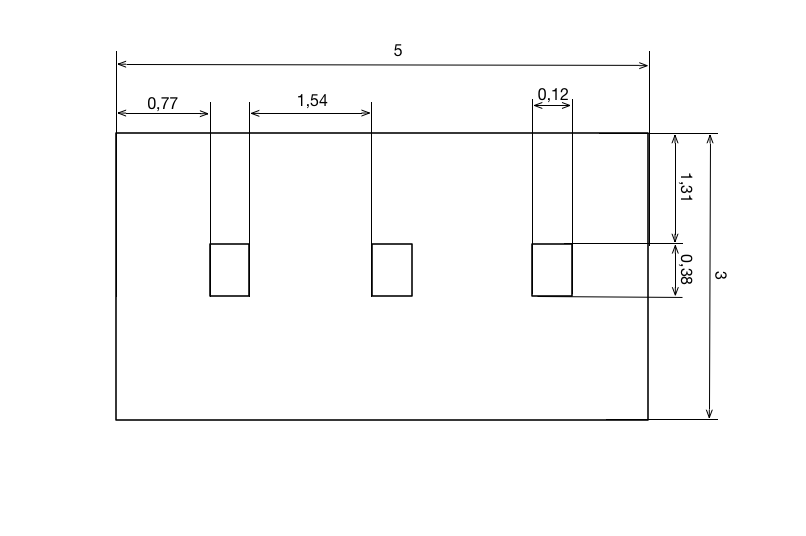
\includegraphics[width=0.8\linewidth]{pics/room.png}}
\caption{Схема расположения светильников в помещении операторов ПЭВМ.}
\label{pic:room}
\end{figure}
\subsection{Утилизация и списание аппаратных комплектующих}
Списание техники организация должна проводить, подтверждая факт утилизации компьютеров и оргтехники. Для организаций эта норма предписана Федеральным законом "Об отходах производства и потребления. То есть, списанная, но не утилизированная техника – это серьезное нарушение закона, не говоря уже об  угрозе окружающей среде.

\subsubsection{Стандартная процедура списания и утилизации техники}
Стандартный процесс списания техники и утилизации компьютерного оборудования включает в себя следующие шаги:
\begin{itemize}
\item Компания, перед которой стоит цель списания техники, создает специальную внутреннюю комиссию. Ее основной задачей будет принятие коллегиального решения о том, какую именно технику уже пора списывать.
\item Решение о списании компьютеров и оргтехники данной комиссии непременно должно базироваться на экспертном заключении. Эксперт может быть как штатным сотрудником компании (обязательно иметь подтверждающие документы по образованию в сфере обслуживания/ремонта данной техники), так и привлеченным извне независимым специалистом. Обязательно потребуется акт технической экспертизы компьютеров или оргтехники, проведенной компанией-производителем, либо другой компанией, имеющее разрешение на обслуживание и ремонт данной техники. Такой акт технической экспертизы компьютеров и оборудования документально подтверждает, что техника неисправна, ее ремонт нецелесообразен и ей пора на  покой. Можно списывать и утилизировать старую технику.
\item Чтобы окончательно завершить списание оргтехники и компьютеров и забыть о  них, придется предоставить еще и документальное подтверждение того, что он  действительно был правильно утилизирован, а не продолжил уничтожать нашу экосистему, распадаясь на тяжелые металлы и ядовитые соединения.

\end{itemize}

Очевидно, что данная процедура списания компьютеров и утилизации оборудования очень долгая и сложная. Правильней было бы заключить договор на утилизацию и перепоручить  утилизацию оборудования специализированной компании.

Компании предлагают услугу вывоза и утилизации компьютерной техники и оргтехники, которая поможет быстро, законно и с минимальными затратами сил и времени избавиться от старой техники. 

После заключения договора, специализированная компания несет ответственность за то, чтобы провести правильное списание оргтехники и корректно выполнить вывоз и утилизацию компьютеров и прочей старой техники.
При утилизации старых компьютеров происходит их разработк
а на фракции: металлы, пластмассы, стекло, провода, штекеры. Из одной тонны компьютерного лома получают до 200 кг меди, 480 кг железа и нержавеющей стали, 32 кг алюминия, 3 кг серебра, 1 кг золота и 300 г палладия.

Переработку промышленных отходов производят на специальных полигонах, создаваемых в соответствии с требованиями СНиП 2.01.28-85 и предназначенных для централизованного сбора обезвреживания и захоронения токсичных отходов промышленных предприятий, НИИ и учреждений.
